
The product is constructed with a number of components, which all have a central role of the final product. They can all be seen in \autoref{fig:sys_dia}. A list of the major components and their function can be seen below  

\begin{itemize}[noitemsep] 
\item \gls{mcu}: The central part of any integrated system, handles all the calculations and the program code.
\item Radio: All the communications with the rest of the world will be handled by the radio, sending on the VHF and UHF band.
\item \gls{imu}: Movement detection is measured with a accelerometer, this to determine if the unit is  in motion or laying still. 
\item \gls{ldo}: A Low-dropout regulator can supply the system with a smoother voltage because no switching is acctualy taking place.
\item Hall sensor: The hall sensor is used as a switch for the system by sensing if a magnet is nearby and then turning off the circuit.
\item \gls{rtc}: A real time clock is important to aquire data at a specific set time, it is important that the clock is exact over the whole life of the pruduct.
\end{itemize} 


\begin{figure}[H] 
\centering 
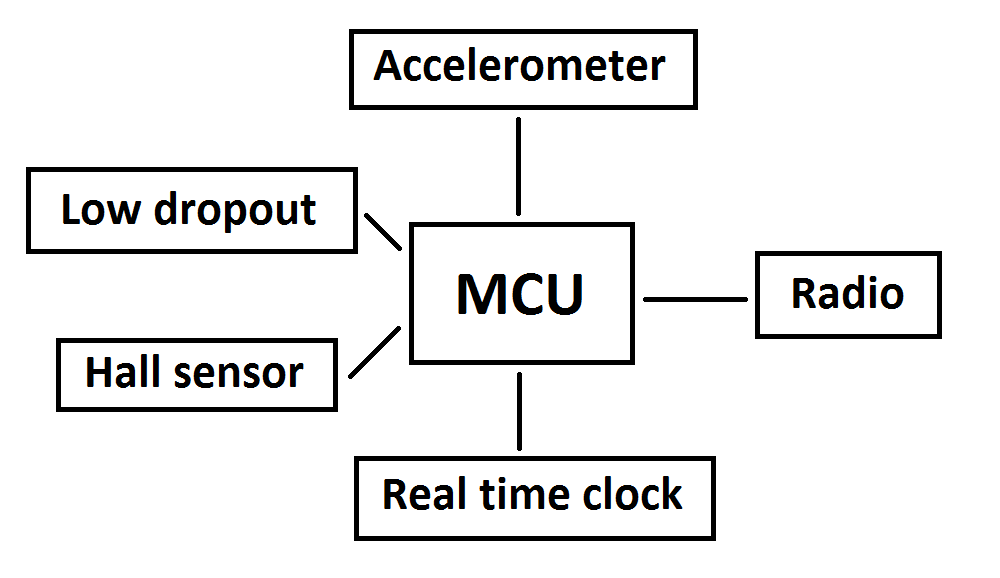
\includegraphics[width=.8\linewidth]{Figures/System_diagram} 
\captionsource{The prototype connection}{Aurthor}
\label{fig:sys_dia} 
\end{figure} 

Each of the components in this project is carfully chosen to get the functionallity and effect that the company is after. To ensure the system works as intended the company have aquired development boards to each of the components. Every components needs to be tested to ensure their induvidial functionallity. Each development board is connected to the micro controllers board. First off the gls{mcu} have to be set up in a correct way with all it parameters and then the other components could be connected and initilized one after another. The whole connection can be seen in \autoref{rattbo}.

%\begin{figure}[H] 
%\centering 
%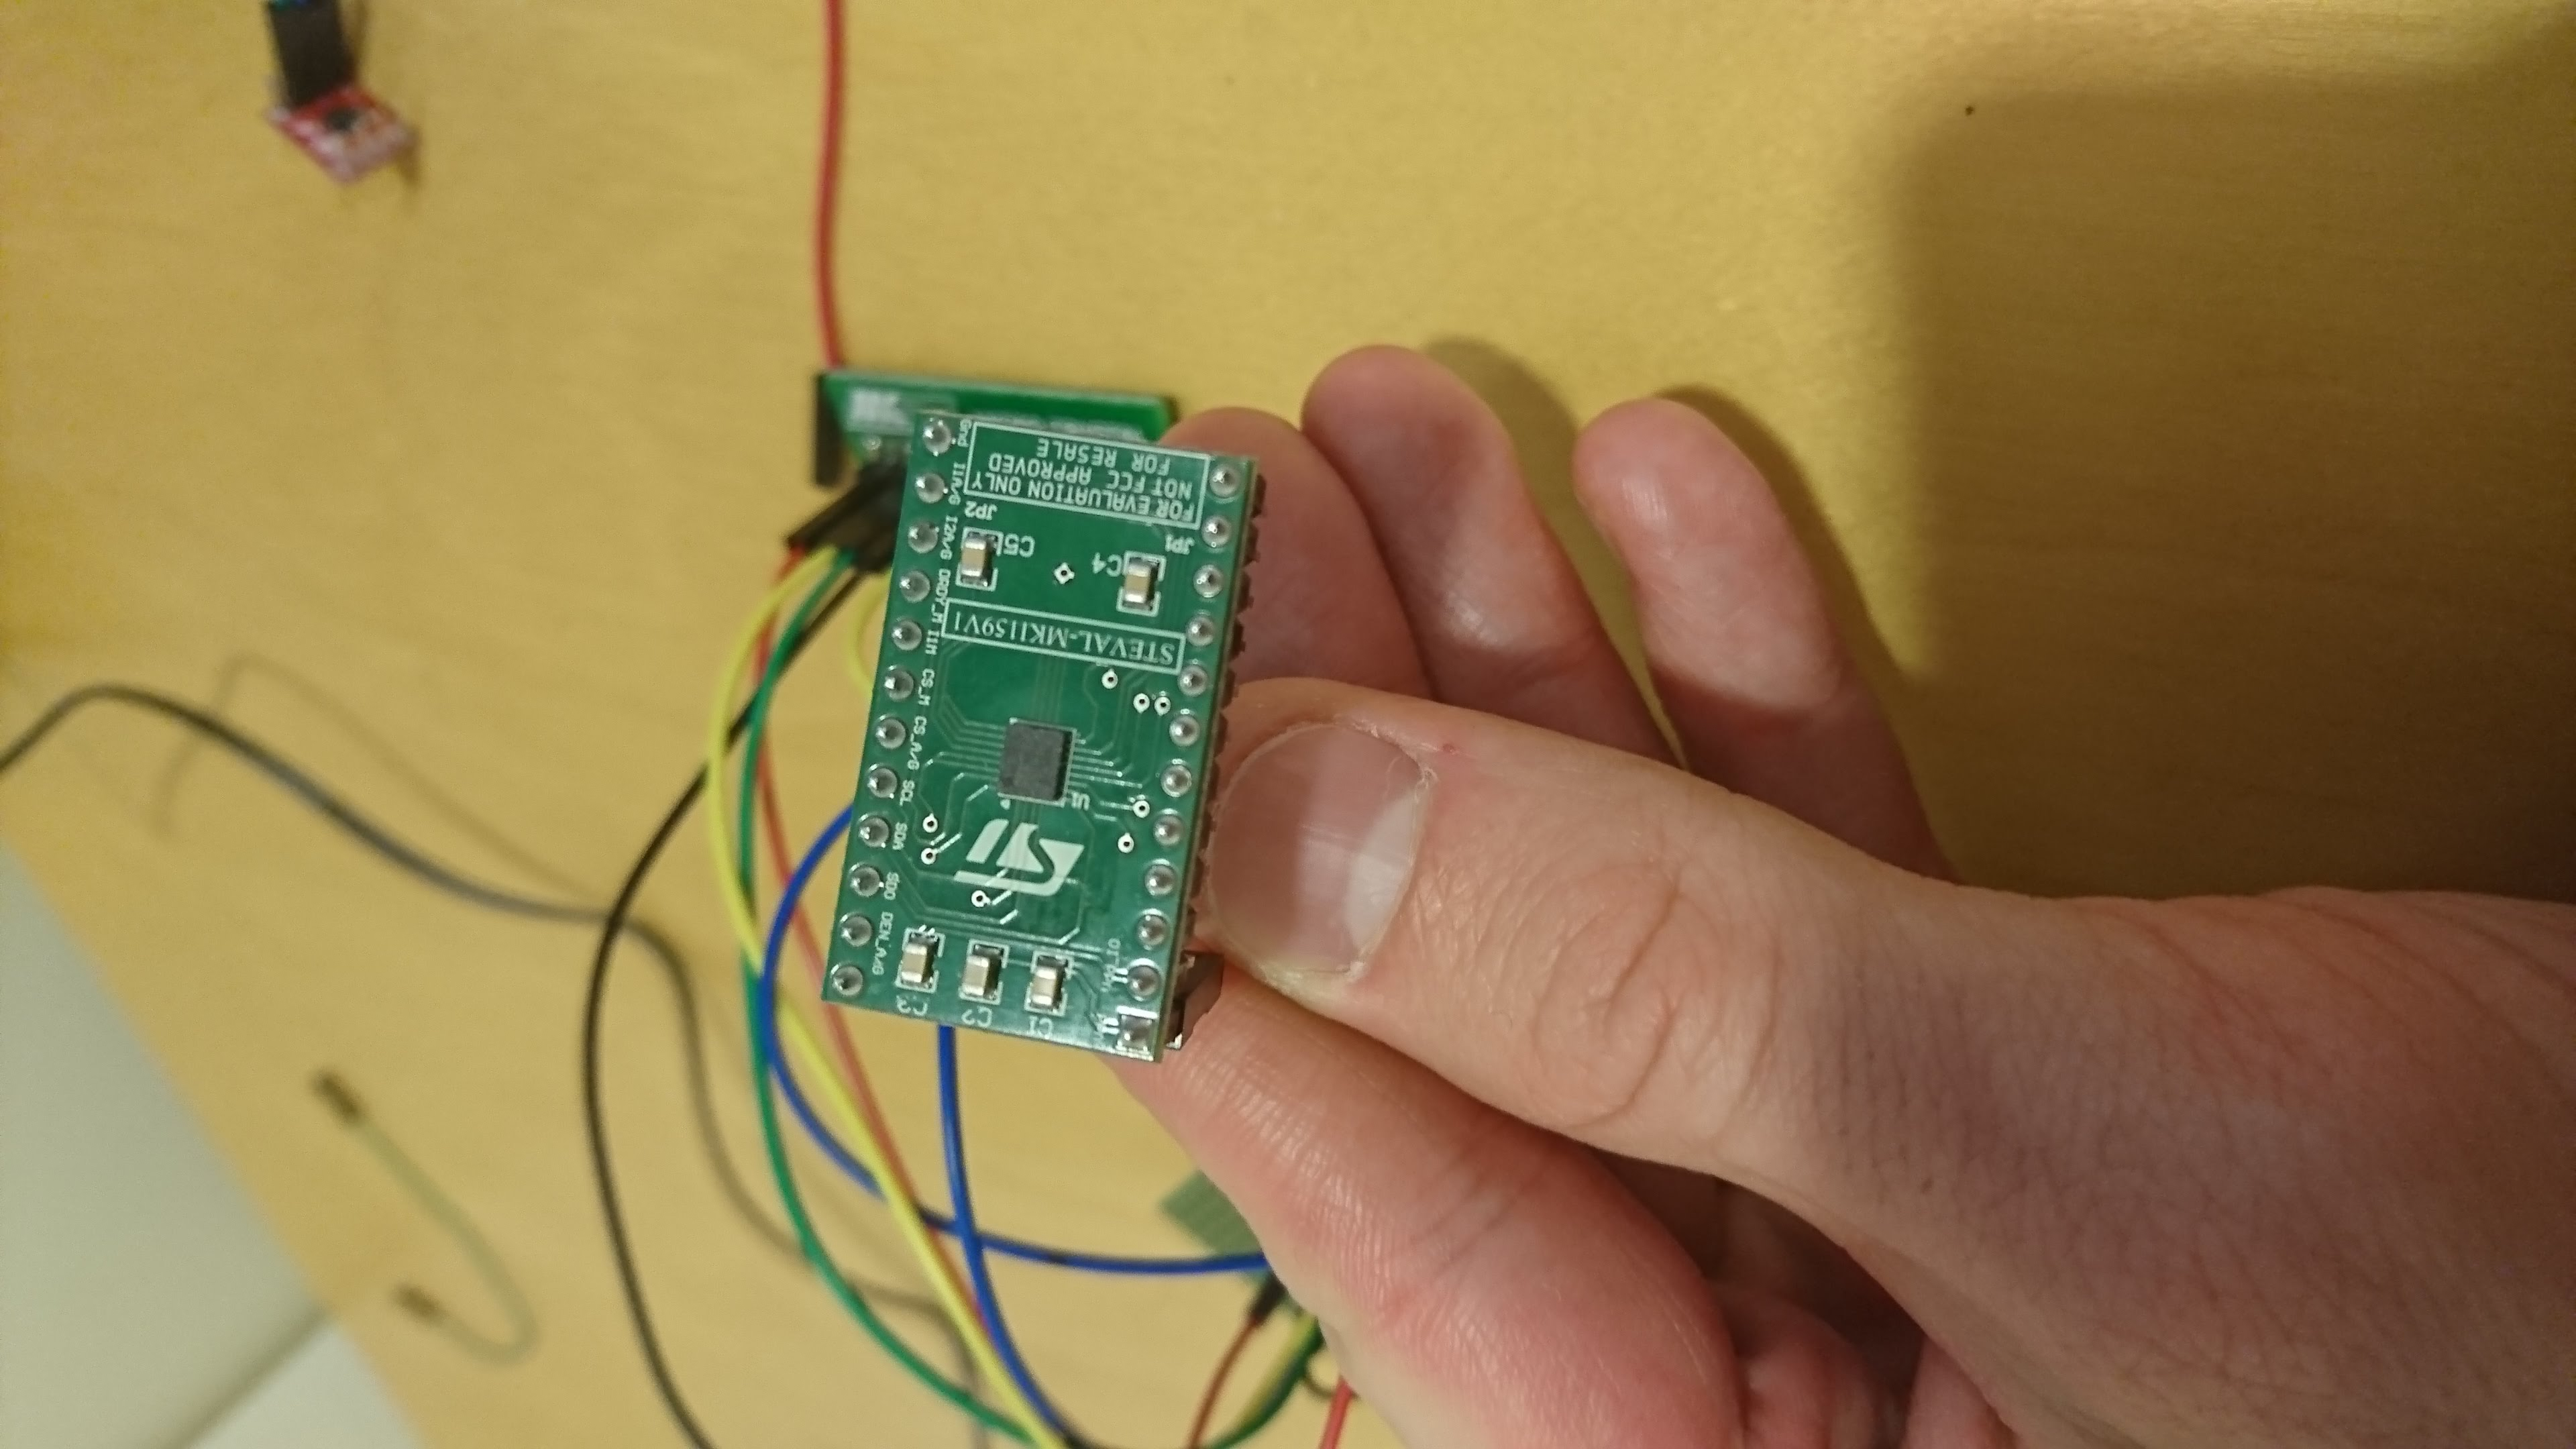
\includegraphics[width=.8\linewidth]{Figures/DSC_0103} 
%\captionsource{The prototype connection}{\url{Aurthor}}
%\label{rattbo} 
%\end{figure} 

The \gls{mcu} can dtad

\subsection{MicroController Unit}
The \gls{mcu} used for this project is a processor type that is used by this company many times before and has been chosen to this project for its small size, low power draw, sufficient connections and feautures. The processor can be determined to have these many connections and enough functionallity. And by choosing between three different variants the chosen chip is the pic18lf46k22\cite{pic18}.
\subsubsection{Power}

The processor do not start up on it own, much consideration needs in making right initzilation and configure it right. Powering it is done by connnecting the VDD pin to the power net. Connected to ground is the Vss pins on the processor. To ensure the current fed is as smooth as possible capacitors are connected between these two pins. The value of these capacitors are directly taken from the datasheet.

\subsubsection{Connenctions}
%% In the registers 
In start of every microcontroller the processor have to be programmed. This is done on the processor by a principle called In Circuit programming\cite{}. Here the most common implementation is the \gls{jtag}, where the all the programming and debugging is done through a standardized interface. The approach is different on this \gls{mcu}, here three pin's is used to program the device. The first one is the "PGC" which is the clock signal for the In-Circuit Debugger and In-Circuit Serial Programming. This is done with the use of 
And that is by connetue

\subsubsection{Software implementation}

\subsection{Accelerometer}
The component used is a 3-axis, ultra-low-powera and high performance accelerometer from ST\cite{STacc}.

\subsubsection{Power}
Two voltage connections is apperent on this device, one which is called VDD and the other is called VDD-IO. 

\subsubsection{Connenctions}
 In the registers 

\subsubsection{Software implementation}

\subsection{Radio}


\subsubsection{Power}


\subsubsection{Connenctions}
 In the registers 

\subsubsection{Software implementation} %% Ändra denna
Radio Chip Waking Up First,  the  radio  is  in  the  off  state. After  the  SDN  pin  is  pulled  low,  the  radio  wakes  up  and  performs  a  Power  on.
Reset  which  takes  a  maximum  of  6 ms  (900 $\mu$ s  typical  at  room  temperature)  until  the  chip  is  ready  to  receive commands on the SPI bus. The GPIO1 pin goes high when the radio is ready for receiving SPI commands. During the reset period, the radio cannot accept any SPI commands. 

